\mbox{$\displaystyle $\,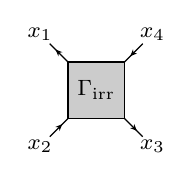
\begin{tikzpicture}[x=0.550cm, y=0.550cm, line width=0.450pt, baseline={([yshift=-0.6ex]0,0)}]
  \draw (0.000,0.000) -- (-0.650,0.650);
  \draw (0.000,0.000) -- (-0.650,-0.650);
  \draw (0.000,0.000) -- (0.650,-0.650);
  \draw (0.000,0.000) -- (0.650,0.650);
  \draw (-0.650,0.650) -- (-1.074,1.074);
  \fill (-0.939,0.939) -- (-0.875,0.780) -- (-0.864,0.864) -- (-0.780,0.875) -- cycle;
  \draw (-0.650,-0.650) -- (-1.074,-1.074);
  \fill (-0.785,-0.785) -- (-0.945,-0.849) -- (-0.860,-0.860) -- (-0.849,-0.945) -- cycle;
  \draw (0.650,-0.650) -- (1.074,-1.074);
  \fill (0.939,-0.939) -- (0.875,-0.780) -- (0.864,-0.864) -- (0.780,-0.875) -- cycle;
  \draw (0.650,0.650) -- (1.074,1.074);
  \fill (0.785,0.785) -- (0.945,0.849) -- (0.860,0.860) -- (0.849,0.945) -- cycle;
  \fill[black!20] (-0.650,-0.650) rectangle (0.650,0.650);
  \draw (-0.650,-0.650) rectangle (0.650,0.650);
  \node[font=\footnotesize, inner sep=0.6pt] at (0.000,0.000) {$\Gamma_{\rm irr}$};
  \node[font=\footnotesize, inner sep=0pt, anchor=315] at (-1.138,1.138) {$x_{1}$};
  \node[font=\footnotesize, inner sep=0pt, anchor=45] at (-1.138,-1.138) {$x_{2}$};
  \node[font=\footnotesize, inner sep=0pt, anchor=135] at (1.138,-1.138) {$x_{3}$};
  \node[font=\footnotesize, inner sep=0pt, anchor=225] at (1.138,1.138) {$x_{4}$};
\end{tikzpicture}}
\diagramgap
\mbox{$\displaystyle +\,$\,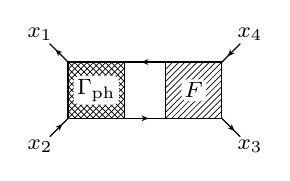
\begin{tikzpicture}[x=0.550cm, y=0.550cm, line width=0.450pt, baseline={([yshift=-0.6ex]0,0)}]
  \draw (-0.475,-0.650) -- (0.475,-0.650);
  \fill (0.079,-0.650) -- (-0.079,-0.582) -- (-0.028,-0.650) -- (-0.079,-0.718) -- cycle;
  \draw (0.475,0.650) -- (-0.475,0.650);
  \fill (-0.079,0.650) -- (0.079,0.582) -- (0.028,0.650) -- (0.079,0.718) -- cycle;
  \draw (1.125,0.000) -- (0.475,0.650);
  \draw (1.125,0.000) -- (0.475,-0.650);
  \draw (1.125,0.000) -- (1.775,-0.650);
  \draw (1.125,0.000) -- (1.775,0.650);
  \draw (-1.125,0.000) -- (-1.775,0.650);
  \draw (-1.125,0.000) -- (-1.775,-0.650);
  \draw (-1.125,0.000) -- (-0.475,-0.650);
  \draw (-1.125,0.000) -- (-0.475,0.650);
  \draw (-1.775,0.650) -- (-2.199,1.074);
  \fill (-2.064,0.939) -- (-2.000,0.780) -- (-1.989,0.864) -- (-1.905,0.875) -- cycle;
  \draw (-1.775,-0.650) -- (-2.199,-1.074);
  \fill (-1.910,-0.785) -- (-2.070,-0.849) -- (-1.985,-0.860) -- (-1.974,-0.945) -- cycle;
  \draw (1.775,-0.650) -- (2.199,-1.074);
  \fill (2.064,-0.939) -- (2.000,-0.780) -- (1.989,-0.864) -- (1.905,-0.875) -- cycle;
  \draw (1.775,0.650) -- (2.199,1.074);
  \fill (1.910,0.785) -- (2.070,0.849) -- (1.985,0.860) -- (1.974,0.945) -- cycle;
  \fill[white] (0.475,-0.650) rectangle (1.775,0.650);
  \draw[line width=0.248pt] (0.475,0.481) -- (0.644,0.650) (0.475,0.340) -- (0.785,0.650) (0.475,0.199) -- (0.926,0.650) (0.475,0.057) -- (1.068,0.650) (0.475,-0.084) -- (1.209,0.650) (0.475,-0.226) -- (1.351,0.650) (0.475,-0.367) -- (1.492,0.650) (0.475,-0.509) -- (1.634,0.650) (0.475,-0.650) -- (1.775,0.650) (0.616,-0.650) -- (1.775,0.509) (0.758,-0.650) -- (1.775,0.367) (0.899,-0.650) -- (1.775,0.226) (1.041,-0.650) -- (1.775,0.084) (1.182,-0.650) -- (1.775,-0.057) (1.324,-0.650) -- (1.775,-0.199) (1.465,-0.650) -- (1.775,-0.340) (1.606,-0.650) -- (1.775,-0.481);
  \begin{scope}
  \clip (0.475,-0.650) rectangle (1.775,0.650);
  \node[font=\footnotesize, inner sep=1.2pt, fill=white, rounded corners=2pt] at (1.125,0.000) {$F$};
  \end{scope}
  \draw (0.475,-0.650) rectangle (1.775,0.650);
  \fill[white] (-1.775,-0.650) rectangle (-0.475,0.650);
  \draw[line width=0.248pt] (-1.775,0.481) -- (-1.606,0.650) (-1.775,0.340) -- (-1.465,0.650) (-1.775,0.199) -- (-1.324,0.650) (-1.775,0.057) -- (-1.182,0.650) (-1.775,-0.084) -- (-1.041,0.650) (-1.775,-0.226) -- (-0.899,0.650) (-1.775,-0.367) -- (-0.758,0.650) (-1.775,-0.509) -- (-0.616,0.650) (-1.775,-0.650) -- (-0.475,0.650) (-1.634,-0.650) -- (-0.475,0.509) (-1.492,-0.650) -- (-0.475,0.367) (-1.351,-0.650) -- (-0.475,0.226) (-1.209,-0.650) -- (-0.475,0.084) (-1.068,-0.650) -- (-0.475,-0.057) (-0.926,-0.650) -- (-0.475,-0.199) (-0.785,-0.650) -- (-0.475,-0.340) (-0.644,-0.650) -- (-0.475,-0.481) (-1.775,-0.481) -- (-1.606,-0.650) (-1.775,-0.340) -- (-1.465,-0.650) (-1.775,-0.199) -- (-1.324,-0.650) (-1.775,-0.057) -- (-1.182,-0.650) (-1.775,0.084) -- (-1.041,-0.650) (-1.775,0.226) -- (-0.899,-0.650) (-1.775,0.367) -- (-0.758,-0.650) (-1.775,0.509) -- (-0.616,-0.650) (-1.775,0.650) -- (-0.475,-0.650) (-1.634,0.650) -- (-0.475,-0.509) (-1.492,0.650) -- (-0.475,-0.367) (-1.351,0.650) -- (-0.475,-0.226) (-1.209,0.650) -- (-0.475,-0.084) (-1.068,0.650) -- (-0.475,0.057) (-0.926,0.650) -- (-0.475,0.199) (-0.785,0.650) -- (-0.475,0.340) (-0.644,0.650) -- (-0.475,0.481);
  \begin{scope}
  \clip (-1.775,-0.650) rectangle (-0.475,0.650);
  \node[font=\footnotesize, inner sep=1.2pt, fill=white, rounded corners=2pt] at (-1.125,0.000) {$\Gamma_{\rm ph}$};
  \end{scope}
  \draw (-1.775,-0.650) rectangle (-0.475,0.650);
  \node[font=\footnotesize, inner sep=0pt, anchor=315] at (-2.263,1.138) {$x_{1}$};
  \node[font=\footnotesize, inner sep=0pt, anchor=45] at (-2.263,-1.138) {$x_{2}$};
  \node[font=\footnotesize, inner sep=0pt, anchor=135] at (2.263,-1.138) {$x_{3}$};
  \node[font=\footnotesize, inner sep=0pt, anchor=225] at (2.263,1.138) {$x_{4}$};
\end{tikzpicture}}
\diagramgap
\mbox{$\displaystyle -\,$\,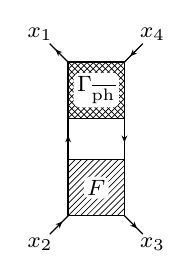
\begin{tikzpicture}[x=0.550cm, y=0.550cm, line width=0.450pt, baseline={([yshift=-0.6ex]0,0)}]
  \draw (0.650,0.475) -- (0.650,-0.475);
  \fill (0.650,-0.079) -- (0.718,0.079) -- (0.650,0.028) -- (0.582,0.079) -- cycle;
  \draw (-0.650,-0.475) -- (-0.650,0.475);
  \fill (-0.650,0.079) -- (-0.718,-0.079) -- (-0.650,-0.028) -- (-0.582,-0.079) -- cycle;
  \draw (0.000,-1.125) -- (-0.650,-0.475);
  \draw (0.000,-1.125) -- (-0.650,-1.775);
  \draw (0.000,-1.125) -- (0.650,-1.775);
  \draw (0.000,-1.125) -- (0.650,-0.475);
  \draw (0.000,1.125) -- (-0.650,1.775);
  \draw (0.000,1.125) -- (-0.650,0.475);
  \draw (0.000,1.125) -- (0.650,0.475);
  \draw (0.000,1.125) -- (0.650,1.775);
  \draw (-0.650,1.775) -- (-1.074,2.199);
  \fill (-0.939,2.064) -- (-0.875,1.905) -- (-0.864,1.989) -- (-0.780,2.000) -- cycle;
  \draw (-0.650,-1.775) -- (-1.074,-2.199);
  \fill (-0.785,-1.910) -- (-0.945,-1.974) -- (-0.860,-1.985) -- (-0.849,-2.070) -- cycle;
  \draw (0.650,-1.775) -- (1.074,-2.199);
  \fill (0.939,-2.064) -- (0.875,-1.905) -- (0.864,-1.989) -- (0.780,-2.000) -- cycle;
  \draw (0.650,1.775) -- (1.074,2.199);
  \fill (0.785,1.910) -- (0.945,1.974) -- (0.860,1.985) -- (0.849,2.070) -- cycle;
  \fill[white] (-0.650,-1.775) rectangle (0.650,-0.475);
  \draw[line width=0.248pt] (-0.650,-0.644) -- (-0.481,-0.475) (-0.650,-0.785) -- (-0.340,-0.475) (-0.650,-0.926) -- (-0.199,-0.475) (-0.650,-1.068) -- (-0.057,-0.475) (-0.650,-1.209) -- (0.084,-0.475) (-0.650,-1.351) -- (0.226,-0.475) (-0.650,-1.492) -- (0.367,-0.475) (-0.650,-1.634) -- (0.509,-0.475) (-0.650,-1.775) -- (0.650,-0.475) (-0.509,-1.775) -- (0.650,-0.616) (-0.367,-1.775) -- (0.650,-0.758) (-0.226,-1.775) -- (0.650,-0.899) (-0.084,-1.775) -- (0.650,-1.041) (0.057,-1.775) -- (0.650,-1.182) (0.199,-1.775) -- (0.650,-1.324) (0.340,-1.775) -- (0.650,-1.465) (0.481,-1.775) -- (0.650,-1.606);
  \begin{scope}
  \clip (-0.650,-1.775) rectangle (0.650,-0.475);
  \node[font=\footnotesize, inner sep=1.2pt, fill=white, rounded corners=2pt] at (0.000,-1.125) {$F$};
  \end{scope}
  \draw (-0.650,-1.775) rectangle (0.650,-0.475);
  \fill[white] (-0.650,0.475) rectangle (0.650,1.775);
  \draw[line width=0.248pt] (-0.650,1.606) -- (-0.481,1.775) (-0.650,1.465) -- (-0.340,1.775) (-0.650,1.324) -- (-0.199,1.775) (-0.650,1.182) -- (-0.057,1.775) (-0.650,1.041) -- (0.084,1.775) (-0.650,0.899) -- (0.226,1.775) (-0.650,0.758) -- (0.367,1.775) (-0.650,0.616) -- (0.509,1.775) (-0.650,0.475) -- (0.650,1.775) (-0.509,0.475) -- (0.650,1.634) (-0.367,0.475) -- (0.650,1.492) (-0.226,0.475) -- (0.650,1.351) (-0.084,0.475) -- (0.650,1.209) (0.057,0.475) -- (0.650,1.068) (0.199,0.475) -- (0.650,0.926) (0.340,0.475) -- (0.650,0.785) (0.481,0.475) -- (0.650,0.644) (-0.650,0.644) -- (-0.481,0.475) (-0.650,0.785) -- (-0.340,0.475) (-0.650,0.926) -- (-0.199,0.475) (-0.650,1.068) -- (-0.057,0.475) (-0.650,1.209) -- (0.084,0.475) (-0.650,1.351) -- (0.226,0.475) (-0.650,1.492) -- (0.367,0.475) (-0.650,1.634) -- (0.509,0.475) (-0.650,1.775) -- (0.650,0.475) (-0.509,1.775) -- (0.650,0.616) (-0.367,1.775) -- (0.650,0.758) (-0.226,1.775) -- (0.650,0.899) (-0.084,1.775) -- (0.650,1.041) (0.057,1.775) -- (0.650,1.182) (0.199,1.775) -- (0.650,1.324) (0.340,1.775) -- (0.650,1.465) (0.481,1.775) -- (0.650,1.606);
  \begin{scope}
  \clip (-0.650,0.475) rectangle (0.650,1.775);
  \node[font=\footnotesize, inner sep=1.2pt, fill=white, rounded corners=2pt] at (0.000,1.125) {$\Gamma_{\overline{\rm ph}}$};
  \end{scope}
  \draw (-0.650,0.475) rectangle (0.650,1.775);
  \node[font=\footnotesize, inner sep=0pt, anchor=315] at (-1.138,2.263) {$x_{1}$};
  \node[font=\footnotesize, inner sep=0pt, anchor=45] at (-1.138,-2.263) {$x_{2}$};
  \node[font=\footnotesize, inner sep=0pt, anchor=135] at (1.138,-2.263) {$x_{3}$};
  \node[font=\footnotesize, inner sep=0pt, anchor=225] at (1.138,2.263) {$x_{4}$};
\end{tikzpicture}}
\diagramgap
\mbox{$\displaystyle -\,\frac{1}{2}$\,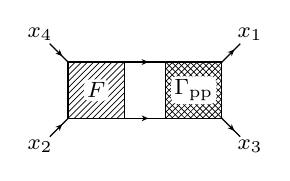
\begin{tikzpicture}[x=0.550cm, y=0.550cm, line width=0.450pt, baseline={([yshift=-0.6ex]0,0)}]
  \draw (-0.475,0.650) -- (0.475,0.650);
  \fill (0.079,0.650) -- (-0.079,0.718) -- (-0.028,0.650) -- (-0.079,0.582) -- cycle;
  \draw (-0.475,-0.650) -- (0.475,-0.650);
  \fill (0.079,-0.650) -- (-0.079,-0.582) -- (-0.028,-0.650) -- (-0.079,-0.718) -- cycle;
  \draw (-1.125,0.000) -- (-1.775,0.650);
  \draw (-1.125,0.000) -- (-1.775,-0.650);
  \draw (-1.125,0.000) -- (-0.475,-0.650);
  \draw (-1.125,0.000) -- (-0.475,0.650);
  \draw (1.125,0.000) -- (0.475,0.650);
  \draw (1.125,0.000) -- (0.475,-0.650);
  \draw (1.125,0.000) -- (1.775,-0.650);
  \draw (1.125,0.000) -- (1.775,0.650);
  \draw (1.775,0.650) -- (2.199,1.074);
  \fill (2.064,0.939) -- (1.905,0.875) -- (1.989,0.864) -- (2.000,0.780) -- cycle;
  \draw (-1.775,-0.650) -- (-2.199,-1.074);
  \fill (-1.910,-0.785) -- (-2.070,-0.849) -- (-1.985,-0.860) -- (-1.974,-0.945) -- cycle;
  \draw (1.775,-0.650) -- (2.199,-1.074);
  \fill (2.064,-0.939) -- (2.000,-0.780) -- (1.989,-0.864) -- (1.905,-0.875) -- cycle;
  \draw (-1.775,0.650) -- (-2.199,1.074);
  \fill (-1.910,0.785) -- (-1.974,0.945) -- (-1.985,0.860) -- (-2.070,0.849) -- cycle;
  \fill[white] (-1.775,-0.650) rectangle (-0.475,0.650);
  \draw[line width=0.248pt] (-1.775,0.481) -- (-1.606,0.650) (-1.775,0.340) -- (-1.465,0.650) (-1.775,0.199) -- (-1.324,0.650) (-1.775,0.057) -- (-1.182,0.650) (-1.775,-0.084) -- (-1.041,0.650) (-1.775,-0.226) -- (-0.899,0.650) (-1.775,-0.367) -- (-0.758,0.650) (-1.775,-0.509) -- (-0.616,0.650) (-1.775,-0.650) -- (-0.475,0.650) (-1.634,-0.650) -- (-0.475,0.509) (-1.492,-0.650) -- (-0.475,0.367) (-1.351,-0.650) -- (-0.475,0.226) (-1.209,-0.650) -- (-0.475,0.084) (-1.068,-0.650) -- (-0.475,-0.057) (-0.926,-0.650) -- (-0.475,-0.199) (-0.785,-0.650) -- (-0.475,-0.340) (-0.644,-0.650) -- (-0.475,-0.481);
  \begin{scope}
  \clip (-1.775,-0.650) rectangle (-0.475,0.650);
  \node[font=\footnotesize, inner sep=1.2pt, fill=white, rounded corners=2pt] at (-1.125,0.000) {$F$};
  \end{scope}
  \draw (-1.775,-0.650) rectangle (-0.475,0.650);
  \fill[white] (0.475,-0.650) rectangle (1.775,0.650);
  \draw[line width=0.248pt] (0.475,0.481) -- (0.644,0.650) (0.475,0.340) -- (0.785,0.650) (0.475,0.199) -- (0.926,0.650) (0.475,0.057) -- (1.068,0.650) (0.475,-0.084) -- (1.209,0.650) (0.475,-0.226) -- (1.351,0.650) (0.475,-0.367) -- (1.492,0.650) (0.475,-0.509) -- (1.634,0.650) (0.475,-0.650) -- (1.775,0.650) (0.616,-0.650) -- (1.775,0.509) (0.758,-0.650) -- (1.775,0.367) (0.899,-0.650) -- (1.775,0.226) (1.041,-0.650) -- (1.775,0.084) (1.182,-0.650) -- (1.775,-0.057) (1.324,-0.650) -- (1.775,-0.199) (1.465,-0.650) -- (1.775,-0.340) (1.606,-0.650) -- (1.775,-0.481) (0.475,-0.481) -- (0.644,-0.650) (0.475,-0.340) -- (0.785,-0.650) (0.475,-0.199) -- (0.926,-0.650) (0.475,-0.057) -- (1.068,-0.650) (0.475,0.084) -- (1.209,-0.650) (0.475,0.226) -- (1.351,-0.650) (0.475,0.367) -- (1.492,-0.650) (0.475,0.509) -- (1.634,-0.650) (0.475,0.650) -- (1.775,-0.650) (0.616,0.650) -- (1.775,-0.509) (0.758,0.650) -- (1.775,-0.367) (0.899,0.650) -- (1.775,-0.226) (1.041,0.650) -- (1.775,-0.084) (1.182,0.650) -- (1.775,0.057) (1.324,0.650) -- (1.775,0.199) (1.465,0.650) -- (1.775,0.340) (1.606,0.650) -- (1.775,0.481);
  \begin{scope}
  \clip (0.475,-0.650) rectangle (1.775,0.650);
  \node[font=\footnotesize, inner sep=1.2pt, fill=white, rounded corners=2pt] at (1.125,0.000) {$\Gamma_{\rm pp}$};
  \end{scope}
  \draw (0.475,-0.650) rectangle (1.775,0.650);
  \node[font=\footnotesize, inner sep=0pt, anchor=225] at (2.263,1.138) {$x_{1}$};
  \node[font=\footnotesize, inner sep=0pt, anchor=45] at (-2.263,-1.138) {$x_{2}$};
  \node[font=\footnotesize, inner sep=0pt, anchor=135] at (2.263,-1.138) {$x_{3}$};
  \node[font=\footnotesize, inner sep=0pt, anchor=315] at (-2.263,1.138) {$x_{4}$};
\end{tikzpicture}}
